\documentclass[table]{beamer}
\usetheme{Madrid} %changeable
\usepackage{animate}
%\documentclass{article}
% \setlength{\arrayrulewidth}{0.5mm}
% \setlength{\tabcolsep}{18pt}
%\renewcommand{\arraystretch}{2.5}
\usepackage{pgfplots} 
\usepackage{tikz}
\usetikzlibrary{positioning}


\title{Introduction to Beamer}
\subtitle{A brief overview}

\author[FTK]{Farhan Tahmidul Karim}
\institute[BUET]
{
    Department of Computer Science \& Engineering\\
    Bangladesh University of Engineering and Technology
}
\date{\today}
\logo{\includegraphics[height=1cm]{cse buet logo.png}}

\AtBeginSection[]
{
    \begin{frame}
    \frametitle{Table of Contents}
    \tableofcontents[currentsection]
    \end{frame}
}

\begin{document}

\maketitle

\section{First Section}

\begin{frame}{Applications of DTW}
    \begin{itemize}
    \item<1-> Spoken Word Recognition %C will appear in all slides of the list from 1
    \item<2-> Detect Sales \& Trend %C++ will come in only slides 2 and 3
    \item<3-> Wearable Fitness Trackers
    \item<4-> Route and ETA Calculation
\end{itemize}
    
\end{frame}

\begin{frame}{Spoken Word Recognition by Matching Sound Pattern}
    \begin{figure}
        \centering
        \begin{subfigure}{\textwidth}
            \includegraphics[width = 0.4\linewidth]{voice 1.png}
            \caption{"Doors and corners, kid. That's where they get you" - v1}
            \label{fig:my_label_1}
        \end{subfigure}
        \begin{subfigure}{\textwidth}
        \includegraphics[width = 0.4\linewidth]{voice 2.png}
        \caption{"Doors and corners, kid. That's where they get you" - v2}
        \label{fig:my_label_2}
        \end{subfigure}
    \end{figure}
\end{frame}

% \tikzstyle{pinnode}=[circle,draw=grey!60,fill=grey!40,very thick, minimum size=3mm]

\begin{frame}{Spoken Word Recognition by Sound Matching Pattern: Euclidian Approach}
    \begin{figure}
        \centering
        \includegraphics[width = 0.8\linewidth, height = 0.7\textheight]{EucMat.png}
        \caption{Failure of Euclidian matching in identifying speech delays/pauses}
        \label{fig:my_label_Euclid}
    \end{figure}
\end{frame}


\begin{frame}{Spoken Word Recognition by Sound Matching Pattern: Using DTW }
\centering
\animategraphics[loop,width=8cm]{2}{dtw-animated-}{0}{11}
\end{frame}

\begin{frame}
    \frametitle{Detecting Sales Trends}
    \begin{table}
    \centering
    \begin{tabular}{|s|p{2cm}|p{2cm}| p{1cm}| p{2cm}|}
        \hline
        \rowcolor{lightgray} \multicolumn{5}{|c|}{Units of each product sold per week} \\
        \hline
        \textbf{Product Code} &\textbf{W1} &\textbf{W2} &\textbf{\dots} &\textbf{W52} \\
        \hline
        \textbf{P1} &11 &12 &\dots &7 \\
        \textbf{P2} &7 &6 &\dots &4 \\
        \textbf{P3} &7 &11 &\dots &3 \\
        \textbf{P4} &12 &8 &\dots &2 \\
        \textbf{P5} &8 &5 &\dots &0 \\
        \textbf{P6} &4 &3 &\dots &10 \\
        \textbf{P7} &5 &6 &\dots &5 \\
        \textbf\dots &\dots &\dots &\dots &\dots \\
        \textbf{P20} &18 &6 &\dots  &7 \\
        \hline
    \end{tabular}
    \caption{\label{demo-table}Weekly sales transaction data set of a company throughout last year}
    \end{table}
\end{frame}

\begin{frame}
    \frametitle{Detecting Sales Trends}
    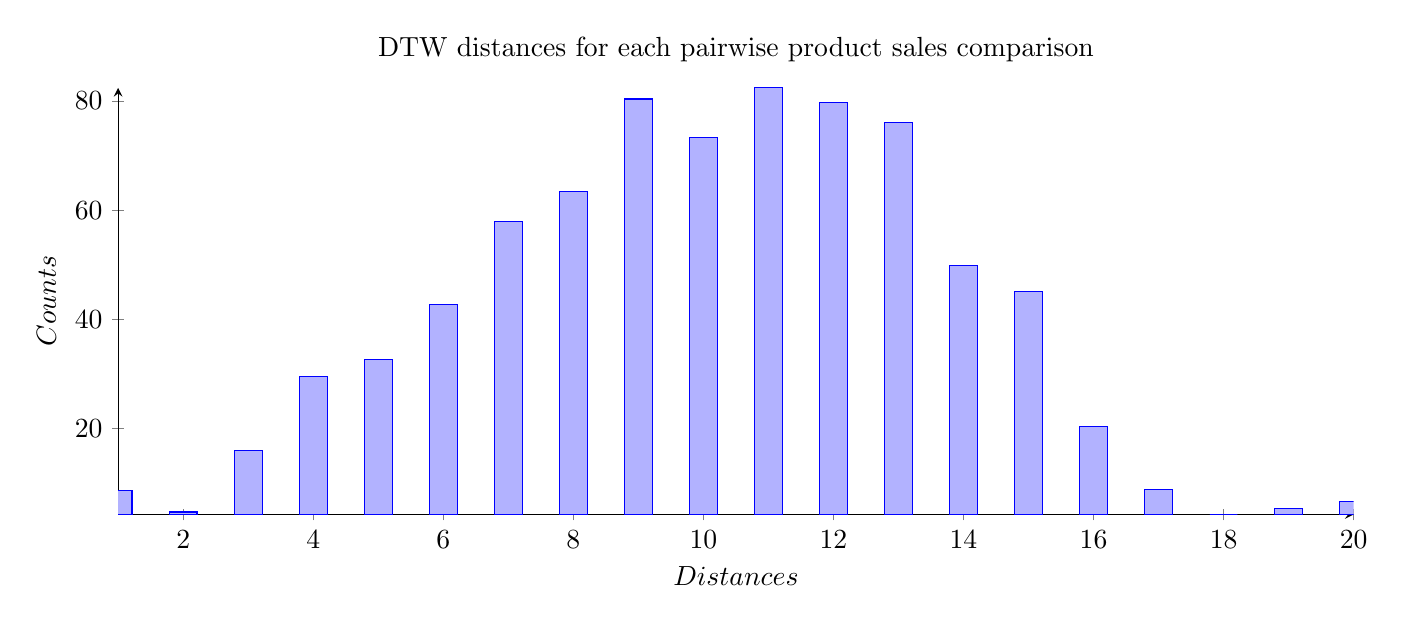
\begin{tikzpicture}
    \begin{axis} [
        title={DTW distances for each pairwise product sales comparison},
        ybar,
        height=7cm,
        width=0.8\paperwidth,
        axis lines = left,
        xlabel = \(Distances\),
        ylabel = {\(Counts\)},
    ]
        \addplot coordinates {
            (1,8.55) 
            (2,4.70) 
            (3,15.90) 
            (4,29.44)
            (5,32.66)
            (6,42.78)
            (7,57.89)
            (8,63.44)
            (9,80.37)
            (10,73.23)
            (11,82.4)
            (12,79.78)
            (13,75.99)
            (14,49.8)
            (15,45.12)
            (16,20.42)
            (17,8.76)
            (18,4.23)
            (19,5.28)
            (20,6.55)
        };
    \end{axis}
\end{tikzpicture}

\end{frame}

\begin{frame}
    \frametitle{Detecting Sales Trends}
    \begin{tikzpicture}
    \begin{axis} [
        title={Comparing Optimal Sales Trend with the Furthest and Closest Products},
        height=6cm,
        width=0.9\paperwidth,
        axis lines = left,
        xlabel = \(Week\),
        ylabel = {\(Sales\)},
        legend style={at={(5,-2)}}
    ]
        \addplot[
            color=blue,
            mark=*,
        ] coordinates {
            (1,12.5)
            (2,13)
            (3,13.5)
            (4,14.2)
            (5,17)
            (6,10)
            (7,15.1)
            (8,16)
            (9,17)
            (10,15.9)
            (11,19.2)
            (12,14.2)
            (13,14.2)
            (14,15)
            (15,10.9)
            (16,20)
            (17,17.8)
            (18,17)
            (19,19.1)
            (20,21)
            (21,19.5)
            (22,15.2)
            (23,16.2)
            (24,16.2)
            (25,15.8)
            (26,15.1)
            (27,19.2)
            (28,19.2)
            (29,20)
            (30,21)
            (31,19.1)
            (32,18)
            (33,17)
            (34,16)
            (35,20)
            (36,19)
            (37,19)
            (38,18)
            (39,17)
            (40,17.6)
            (41,26)
            (42,25)
            (43,16.2)
            (44,23)
            (45,20.8)
            (46,19.5)
            (47,28)
            (48,18)
            (49,19.2)
            (50,15.5)
            (51,21)
            (52,23)
        };
        \legend{Optimal Sales Trend}
        \addplot [
            color=green,
            mark=10-pointed star,
        ] coordinates {
            (1,2)
            (2,0.5)
            (3,4.5)
            (4,0)
            (5,2)
            (6,5)
            (7,5)
            (8,1)
            (9,3)
            (10,2.5)
            (11,1)
            (12,1)
            (13,1)
            (14,1)
            (15,8)
            (16,5)
            (17,3)
            (18,6)
            (19,3)
            (20,6)
            (21,7)
            (22,5)
            (23,4.2)
            (24,4.2)
            (25,10)
            (26,7)
            (27,3)
            (28,5)
            (29,7)
            (30,4.5)
            (31,4.5)
            (32,1)
            (33,2)
            (34,3)
            (35,5.8)
            (36,4.5)
            (37,5.8)
            (38,5.8)
            (39,5.8)
            (40,4.5)
            (41,8)
            (42,7.4)
            (43,7.4)
            (44,6)
            (45,5)
            (46,5)
            (47,5)
            (48,7)
            (49,7)
            (50,5)
            (51,9)
            (52,10)
        };
        \legend{Optimal Sales Trend, P18 (Closest to optimal)}
        \addplot [
            color=orange,
            mark=triangle,
        ] coordinates {
            (1,1)
            (2,0)
            (3,0)
            (4,0.5)
            (5,1.5)
            (6,0)
            (7,0)
            (8,0)
            (9,0)
            (10,1)
            (11,1.2)
            (12,1.4)
            (13,0.6)
            (14,0)
            (15,0)
            (16,0)
            (17,0)
            (18,0)
            (19,0)
            (20,0)
            (21,0.5)
            (22,2)
            (23,1.5)
            (24,1.1)
            (25,2.5)
            (26,0.5)
            (27,0)
            (28,3.4)
            (29,1)
            (30,1.2)
            (31,0.5)
            (32,0)
            (33,0)
            (34,2)
            (35,1.2)
            (36,1.1)
            (37,1.3)
            (38,1.9)
            (39,2)
            (40,0)
            (41,2.5)
            (42,1.2)
            (43,1)
            (44,0)
            (45,0)
            (46,0)
            (47,0)
            (48,1)
            (49,1)
            (50,1.5)
            (51,0)
            (52,0.4)
        };
        \legend{Optimal Sales Trend, P18 (Closest to optimal, P11 (Furthest to optimal)}
    \end{axis}
\end{tikzpicture}
    
\end{frame}

\begin{frame}{Applications of DTW} 
    
    
\end{frame}

\end{document}
